\section{Facility}\label{sec_fac}
The Muon Accelerator Programme (MAP) has developed a concept for the muon collider, shown in Figure~\ref{fig_muon:sketch}. This concept serves as the starting point for the baseline concept and a seed for the tentative parameters in the design studies initiated by the International Muon Collider Collaboration (IMCC)~\cite{IMCC}. The tentative target parameters are reported in Table~\ref{MC:t:param}.

This section describes the physical principles that motivate the present baseline design and outlines promising avenues that may yield improved performances or efficiency. Technical issues are also highlighted. Section~\ref{sec:fac_design_overview} provides an overview of the overall design concept. An approximate expression for luminosity is derived in some detail, as this motivates many of the design choices. Consideration of attainable energy, facility scale and power requirements are described. Possible upgrade schemes and timescales are outlined. The detailed description of design concepts and technical issues surrounding each subsystem are reported in Sections~\ref{sec:fac_proton_driver} -- \ref{sec:fac_collider}, describing the proton source, target, front end, muon cooling system, acceleration and collider in turn. The concepts and technologies developed for the muon collider will require technical demonstration, to be achieved by a number of demonstrator facilities described in Section~\ref{sec:fac_demonstrators}. Section~\ref{sec:fac_synergies} is devoted to the synergies between the R\&{D} programme for the muon collider and the one of other muon-beam facilities. We summarise our conclusions in Section~\ref{sec:conc_out}.

\begin{figure*}
\includegraphics[width=0.75\textwidth, trim={0cm 0 0 0}]{figures/facility/THPAB017f1.pdf}
\centering\textbf{}
\caption{A conceptual scheme for a muon collider.}
\label{fig_muon:sketch}
\end{figure*}

\subsection{Design overview}
\label{sec:fac_design_overview}
Most muon collider designs foresee that muons are created as a product of a high power proton beam incident on a target. Most muons are produced by decay of pions created in the target. In order to capture a large number of negatively and positively charged secondary particles over a broad range of momenta, a solenoid focusing system is used rather than the more conventional horn-type focusing. Following the target the beam is cleaned and most pions decay leaving a beam composed mostly of muons. The muons are captured longitudinally in a sequence of RF cavities arranged to manipulate the single short bunch with large energy spread into a series of bunches each with a much smaller energy spread. 

Following creation of a bunch train, the beam is split into the different charge species and each charge species is cooled separately by a 6D ionisation cooling system. Ionisation cooling increases the beam brightness and hence luminosity. An initial cooling line reduces the muon phase space volume sufficiently that each bunch train can be remerged into a single bunch. Further cooling then reduces the longitudinal and transverse beam size. Final cooling systems for each charge species results in a beam suitable for acceleration and collision.

Ionisation cooling is chosen as it operates on a time scale that is competitive with the muon lifetime. Despite the short time scale, a significant number of muons are lost due to muon decay as well as transmission losses. Nonetheless the increased beam brightness provided by the cooling system yields a significant increase in luminosity.

The beam is then accelerated. Rapid acceleration is required in order to maintain an acceleration time that is much shorter than the muon lifetime in the laboratory frame. Satisfactory yields may be achieved by leveraging the muon lifetime increase during acceleration due to Lorentz time dilation to maximise the acceleration efficiency $\eta_\tau$. The number of muons $N$ changes with time $t$ according to
\begin{equation}
\frac{dN}{dt} = -\frac{m_\mu N c^2}{E \tau_\mu}\,,
\end{equation}
where $m_\mu$, $E$ and $\tau_\mu$ are the muon mass, energy and lifetime respectively. Assuming the muons are travelling, near to the speed of light $c$, through a mean field gradient $\bar{V}$, their energy changes as $dE/dt=e\bar{V}c$, where $e$ is the muon charge. We thus find
\begin{equation}
\frac{dN}{dE} = - \frac{N}{\delta_\tau E} \,,
\end{equation}
where $\delta_\tau = e\bar{V} \tau_\mu/m_\mu c$ is the mean change in energy in one muon lifetime, normalised to the muon rest energy. Integrating yields the acceleration efficiency
\begin{equation}
\eta_\tau =  \frac{N_\pm}{N_{0\pm}} =  \prod_i \left(\frac{E_{i+1}}{E_{i}}\right)^{-1/\delta_{\tau,i}}\,,
\end{equation}
where the product is taken over all accelerator subsystems. Mean gradients $\bar{V} \sim O(1-10)$ MV/m are possible, with higher gradients available in the early parts of the accelerator chain, yielding $\delta_\tau \sim O(10)\gg1$. Muons can thus be accelerated faster than they decay, entailing a limited loss of muons during the acceleration process. 

At low energy rapid acceleration is achieved using a linear accelerator, in order to maximise the average accelerating gradient in this relatively short section. At higher energies recirculation may be used to improve the system efficiency, for example in a dogbone recirculator. Finally, a sequence of pulsed synchrotrons bring the beam up to final energy. Synchrotrons that employ a combination of fixed high-field, superconducting dipoles and lower field pulsed dipoles are under study. The muons are eventually transferred into a low circumference collider ring where collisions occur.

\subsubsection{Luminosity}
\label{sec:luminosity}
The muon collider benefits from significant luminosity even at high energies. Many of the design parameters for a muon collider are driven by the need to achieve a good luminosity. An approximate expression for luminosity may be derived to inform design choices and highlight the critical parameters for optimisation. In particular proton sources are a relatively well-known technology, with examples such as SNS and JPARC in a similar class to the proton driver required for the muon collider. Muon beam facilities comparable to the muon collider have instead never been constructed. In order to quantify the required performance for a muon collider facility, it is convenient to express the luminosity in terms of the proton source parameters and muon facility performance indicators, for example the final muon energy, muon collection efficiency and muon beam quality.

\begin{table*}
\begin{center}
  \begin{tabular}{|*6{c|}}
    \hline
    Parameter & Symbol & Unit &\multicolumn{3}{c|}{Target value} \\
    \hline
    Centre-of-mass energy & $E_\text{cm}$ & \si{\tera\electronvolt} & 3 & 10 & 14 \\
    Luminosity & $\mathfrak{L}$ & \SI{e34}{\per\square\centi\meter\per\second} & 2 & 20 & 40 \\
    Collider circumference& $C_\text{coll}$ & \si{\kilo\meter} & 4.5 & 10 & 14 \\
    \hline
    Muons/bunch & $N_{\pm}$ & \num{e12} & 2.2 & 1.8 & 1.8 \\
    Repetition rate & $f_\text{r}$ & \si{\hertz} & 5 & 5 & 5 \\
    Total beam power  & $P_{_-}+P_{_+}$ & \si{\mega\watt} & 5.3  & 14 &20 \\
    Longitudinal emittance& $\varepsilon_\text{l}$ & \si{\mega\electronvolt\meter} & 7.5 & 7.5 & 7.5 \\
    Transverse emittance& $\varepsilon_\perp$ & \si{\micro\meter} & 25 & 25 & 25 \\
    \hline
    IP bunch length& $\sigma_z $ & \si{\milli\meter} & 5 & 1.5 & 1.1 \\
    IP beta-function& $\beta^*_{\perp} $ & \si{\milli\meter} & 5 & 1.5 & 1.1 \\
    IP beam size& $\sigma_{\perp} $ & \si{\micro\meter} & 3 & 0.9 & 0.6 \\
    \hline
  \end{tabular}
\end{center}
\caption{\label{MC:t:param}Tentative target parameters for MuCs of different
  energies based on the MAP design with modifications. \\[-3pt] \ }
\end{table*}

In each beam crossing in a collider the integrated luminosity increases by \cite{Wolski:2014lba}
\begin{equation}
\Delta \mathfrak{L} = \frac{N_{+,j} N_{-,j}}{4\pi\sigma^2_\perp}\,,
\end{equation}
where $N_{\pm,j}$ are the number of muons in each positively and negatively charged bunch on the $j^{th}$ crossing and $\sigma_\perp$ is the geometric mean of the horizontal ($x$) and vertical ($y$) RMS beam sizes, assumed to be the same for both charge species.

The number of particles in each beam on the $j^{th}$ crossing decreases due to muon decay as 
\begin{equation}
N_{\pm,j} = N_{\pm} \exp(-2 \pi R j/(c\gamma \tau_\mu))\,,
\end{equation}
where $R$ is the collider radius and $\gamma$ the Lorentz factor of the muons. If the facility has a repetition rate of $f_r$ acceleration cycles per second and $n_b$ bunches circulate in the collider, the luminosity will be
\begin{equation}
\mathfrak{L} = f_r n_b \frac{N_{+} N_{-}}{4\pi\sigma^2_\perp} \sum^{j_\text{max}}_{j=0} \exp\left(-\frac{4\pi R}{\gamma c \tau_\mu} j\right)\,.
\end{equation}
For the designs discussed here the muon passes around the collider ring many times ($j_\text{max}\to\infty$) so we can sum the geometric series. Furthermore, $2 \pi R/(c\gamma \tau_\mu)\ll1$, therefore to a good approximation
\begin{equation}
\mathfrak{L} \approx f_r n_b \frac{N_{+} N_{-}}{(4\pi)^2\sigma^2_\perp} \frac{\gamma c \tau_\mu}{R}\,.
\end{equation}
The average collider radius $R$, in terms of the average bending field $\bar{B}$, is $R = p/(e\bar{B}) \approx \gamma m_\mu c / (e\bar{B})$ and
\begin{equation}
\mathfrak{L} \approx f_r n_b \frac{N_{+} N_{-}}{(4\pi)^2\sigma^2_\perp} \frac{\tau_\mu e \bar{B}}{m_\mu}.
\end{equation}

The transverse beam size $\sigma_\perp$ may be expressed in terms of the beam quality (emittance) and the focusing provided by the magnets. $\varepsilon_\perp$ and $\varepsilon_l$ are the normalised emittances in transverse and longitudinal coordinates; a small $\varepsilon$ indicates a beam occupying a small region in position and momentum phase space. To a good approximation $\varepsilon$ is conserved during acceleration. The degree to which the beam is focused is denoted by the lattice Twiss parameter $\beta^*_\perp$. For a short bunch
\begin{equation}\label{sp0}
\sigma_\perp = \sqrt{\frac{m_\mu c \beta^*_\perp \varepsilon_\perp}{p}}\,.
\end{equation}
Stronger lenses create a tighter focus and make the beam size smaller at the interaction point, reducing $\beta^*_\perp$. The minimum beam size is practically limited by the ``hourglass effect''; when the focal length of the lensing system is much shorter than the length of the beam itself, the average beam size at the crossing is dominated by particles that are not at the focus \cite{Chao:2013rba}. For example, when the RMS bunch length is not zero, but $\sigma_z = \beta^*_\perp$, eq.~(\ref{sp0}) is replaced by 

\begin{equation}
\sigma_\perp = \sqrt{\frac{m_\mu c \sigma_z \varepsilon_\perp}{p f_{hg}}}\,,
\end{equation}
with a hourglass factor $f_{hg} \approx 0.76$. The RMS longitudinal emittance is $\varepsilon_l = \gamma m_\mu c^2 \sigma_\delta \sigma_z$ where $\sigma_\delta$ is the fractional RMS energy spread, so the luminosity may be expressed as
\begin{equation}
\mathfrak{L} \approx \frac{e \tau_\mu}{(4 \pi m_\mu c)^2} \frac{f_{hg} \sigma_\delta \bar{B}}{\varepsilon_\perp \varepsilon_L} {E_\mu}^2 N_+ N_- n_b f_r \,,
\end{equation}
where $E_\mu=\gamma m_\mu c^2$ is the energy of the collding muons.

Naively, the number of muons reaching the accelerator may be obtained from the number and energy of protons, i.e. from the proton beam power. This assumes proton energy is fully converted to pions and the capture and beam cooling systems have no losses. In reality pion production is more complicated; practical constraints such as pion reabsorption, other particle production processes and geometrical constraints in the target have a significant effect. Decay and transmission losses occur in the ionisation cooling system that significantly degrades the efficiency.

The final number of muons per bunch in the collider, $N_\pm$, can be related to the proton beam power on target $P_p$ and the conversion efficiency per proton per unit energy $\eta_\pm$ by 
\begin{equation}
N_{\pm} =\frac{\eta_\tau \eta_\pm P_p}{n_b f_r}.
\end{equation}

Overall the luminosity may be expressed as
\begin{equation}
\label{lumform}
\mathfrak{L} \approx 
\underbrace{
    \frac{e \tau_\mu}{(4 \pi m_\mu c)^2}
}_{K_L} 
\frac{f_{hg} \sigma_\delta \bar{B}}{\varepsilon_\perp \varepsilon_L n_b f_r}
\underbrace{
    \eta_+ \eta_- (\eta_\tau P_p E_\mu)^2 
    \vphantom{\frac{e \tau_\mu }{(m_\mu)^2}} % forces vertical alignment of the underbrace
}_{P_+ P_-}\,,
\end{equation}
where $K_L = 4.38 \times 10^{36} \mathrm{ \: MeV \: MW^{-2} \: T^{-1} \: s^{-2}} $ and $P_\pm$ is the muon beam power per species.

This luminosity dependence yields a number of consequences. The luminosity improves approximately with the square of energy at fixed average bending field. We thus find the desired scaling in eq.~(\ref{lums}) that entails, as discussed in the previous section, a constant rate for very massive particles pair-production, as well as a growing VBF rate for precision measurements. The quadratic scaling of the luminosity with energy is peculiar of muon colliders and it is not present, for example, in a linear collider. This is because the beam can be recirculated many times through the interaction point and beamstrahlung has a negligible affect on the focusing that may be achieved at the interaction point of the muon collider. This yields an improvement in power efficiency with energy.

The luminosity is highest for collider rings having strong dipole fields (large $\bar{B}$), so that the circumference is smaller and muons can pass through the interaction region many times before decaying. For this reason a separate collider ring with the highest available dipole fields is proposed after the final acceleration stage, as in Figure~\ref{fig_muon:sketch}.

The luminosity is highest for a small number of very high intensity bunches. The MAP design demanded a single muon bunch of each charge, which yields the highest luminosity per detector. Such a design would enable detectors to be installed at two interaction points. % shiltsev

The luminosity decreases linearly with the facility repetition rate, assuming a fixed proton beam power. For the baseline design, a low repetition rate has been chosen relative to equivalent pulsed proton sources.

The luminosity decreases with the product of the transverse and longitudinal emittance. It is important to achieve a low beam emittance in order to deliver satisfactory luminosity, while maintaining the highest possible efficiency $\eta_\pm$ of converting protons to muons.

Based on these considerations, an approximate guide to the luminosity normalised to beam power is shown in Figure~\ref{fig_muon:power_luminosity} and compared with the one of CLIC.

\subsubsection{Facility size}

\begin{figure}
\centering
\includegraphics[width=0.45\textwidth, trim={0 0 0 0}]{figures/facility/beam_power_lumi1.pdf}
\centering
\caption{MuC luminosity normalised to the muon beam power and compared to CLIC, for different beam energies.}
\label{fig_muon:power_luminosity}
\end{figure}

The geometric dimensions of the MuC depend on future technology and design choices. Some indication of the dimensions can be estimated. The facility scale is expected to be driven by the pulsed synchrotrons in the acceleration system.

The rapid pulsing required in the synchrotrons precludes the use of high-field ramped superconducting magnets such as those used in the LHC. Static high-field superconducting dipoles are proposed combined with rapidly pulsed low-field dipoles. As the beam accelerates the pulsed dipoles are ramped, enabling variation of the mean dipole field. The static dipoles provide a relatively compact and efficient bend. 

Preliminary estimates indicate that acceleration up to 3~TeV centre-of-mass energy, assuming 10~T static dipoles and pulsed dipoles with a field swing $\pm$1.8~T, would require a ring of circumference around 10~km. Around 60~\% of the ring is estimated to be required for pulsed and static bending dipoles. Acceleration up to 10~TeV centre-of-mass energy would require 16~T static dipoles, which are only expected to become available later in the century,  and an approximately 70~\% dipole packing fraction. A 10~TeV facility could be implemented as an upgrade to the 3~TeV facility, as discussed below. Estimates indicate that a ring circumference of up to 35~km may be required. Tuning to accommodate the beam into existing infrastructure such as the 26.7~km circumference LHC tunnel is possible, for example by changing the energy swing in each ring so that more or less space is required for pulsed dipoles. Options that have a fixed dipole field that varies radially in the same superconducting magnet are under study, which may enable an increased average dipole field to be considered.

\subsubsection{Wall-plug power requirements}
The power usage of future accelerator facilities, often referred to as the `wall-plug power', is of great concern and in future may be a stronger practical constraint than the financial cost. The goal is to remain at a wall-plug power consumption for the 10~TeV MuC well below the level estimated for CLIC at 3~TeV (550~MW) or FCC-hh (560~MW). This seems readily achievable; the facility length is considerably shorter than other proposed colliders. Reuse of magnets and RF should make the facility more efficient than linear colliders while the lower energy requirement should result in lower power requirements than hh colliders. The design has to advance more to assess the power consumption scale in a robust fashion.

Muon beam production imposes a fixed power consumption requirement. In particular, the muon cooling system requires several GeV of acceleration in normal conducting cavities at high gradient. Additional power consumption arises from the proton source and cooling plant for the target and other cryogenic systems.

A number of key components drive the power consumption as one extends to high energy:
\begin{itemize}
\item The power loss in the fast-ramping magnets of the pulsed synchrotron and their power converter.
\item The cryogenics system that cools the superconducting
magnets in the collider ring. This depends on the efficiency of shielding the magnets from the muon decay-induced heating.
\item The cryogenics power to cool the superconducting magnets and RF cavities in the pulsed synchrotrons.
\item The power to provide the RF for accelerating cavities in the pulsed synchrotrons.
\end{itemize}
The first contribution requires particular study as it depends on unprecedented large-scale fast ramping systems. The second and third contributions require optimisation of the volume reserved for shielding as compared to magnetised volume. The contributions can be estimated reliably following a suitable design and optimisation of the relevant equipment.

\begin{figure*}[t]
\begin{minipage}{0.47\textwidth}
\begin{center}
\includegraphics[width=\textwidth,trim={100 0  170 0}, clip]{figures/facility/schematic_ppt_3_TeV_stage.pdf}
\end{center}
\end{minipage}
\hfill
\begin{minipage}{0.47\textwidth}
\begin{center}
\includegraphics[width=\textwidth,trim={110 0  160 0}, clip]{figures/facility/schematic_ppt_10_TeV_stage.pdf}
\end{center}
\end{minipage}
\caption{A schematic of a possible staged approach to a muon collider. The first stage, shown on the left, would produce collisions at 3 TeV center-of-mass energy while the second would produce collisions at 10 TeV centre-of-mass energy. Sections of the facility that are not required are shown in grey.
\label{fig_muon:upgrade}}
\end{figure*}

In summary power consumption follows a relation
\begin{equation}
P = P_{src} + P_{linac} + P_{rf} + P_{rcs}+P_{coll}\,,
\end{equation}
where $P_{src}$ is the power needed for the muon source, which is constant with energy, $P_{linac}$ is the power requirement for the linac, which is fixed by the transition energy between the linacs and RCS (Rapid Cycling Synchrotron). $P_{rf}$ is the power requirement for RCS and collider RF cavities, which is approximately proportional to the beam energy, $P_{rcs}$ is the power requirement for the RCS magnets which is likely to rise slowly with energy due to the lower losses associated with slower ramping at high energy and $P_{coll}$ is the power requirement for the collider ring, which is approximately proportional to the collider length i.e. proportional to the beam energy. Overall, the power requirement is expected to rise slightly less than linearly with energy and hence the wall-plug power is expected to be approximately proportional to the beam power.

\subsubsection{Upgrade scheme}

The muon collider can be implemented as a staged concept providing a road
toward higher energies. One such staging scenario is shown in Figure~\ref{fig_muon:upgrade}. The accelerator chain can be expanded by an additional accelerator ring for each energy stage. A new collider ring is required for each energy stage. It may be possible to reuse the magnets and other equipment of the previous collider ring, for example in the new accelerator ring.

Currently, the focus of studies is on 10~TeV. This energy is well beyond the 3~TeV of the third and highest energy stage of CLIC, the highest energy $\mathrm{e^+e^-}$ collider proposal to reach a mature design. A potential intermediate energy of 3~TeV is envisaged at this moment. Its physics case is similar to the final stage of CLIC and it is expected that this stage would roughly cost half as much as the 10~TeV stage~\cite{Roser:2022sht}.

A 3~TeV stage is less demanding in several technological areas. It may not be necessary to implement a mechanical neutrino flux mitigation system in the collider ring arcs; moving the beam inside of the magnet apertures may be sufficient. The final focus magnets require an aperture and a gradient comparable to the values for HL-LHC. In general, it will be possible to implement larger margins in the design at 3~TeV. The operational experience will then allow to accept smaller margins at 10~TeV.

The strength of the collider ring dipoles is crucial for determining the ring size and luminosity. The cost optimum is given by the magnet and tunnel cost; it is possible that cheaper, well established magnet technology---such as NbTi at this moment--- would result in a lower cost even if the tunnel has to be longer. For fixed beam current, the luminosity is proportional to the magnet field and is one aspect of the optimisation.

Once the cost scale of the muon collider concept is more precisely known and once the mitigation of the technical challenges are well defined, the energy staging may be reviewed taking into account the physics case and additional considerations from the site and reuse of existing equipment and infrastructure, such as the LHC tunnel, making possible a high-impact and sustainable physics programme with each upgrade manageable in terms of cost and technical feasibility.

\begin{figure*}
        \includegraphics[width=0.7\textwidth, trim={0 0 0 0}]
        {figures/facility/timeline_1.pdf}
        \centering\textbf{}

\caption{A technically limited timeline for the muon collider R\&D programme that would see a 3 TeV muon collider constructed in the 2040s.}
\label{fig_muon:RDtimeline}
\end{figure*}

\subsubsection{Timeline}
A muon collider with a centre-of-mass energy around 3~TeV could be delivered on a time scale compatible with the end of operation of the HL-LHC. A technically limited timeline is shown in Figure~\ref{fig_muon:RDtimeline} and discussed in greater detail in \cite{Schulte:2022cbw}. The muon collider R\&D programme will consist of the initial phase followed by the conceptual and the technical design phases. The initial phase will establish the potential of the muon collider and the required R\&D programme for the subsequent phases. 

The performance and cost of the facility would be established in detail. A programme of test stands and prototyping of equipment would be performed over a five-year period, including a cooling cell prototype and the possibility of beam tests in a cooling demonstrator. This programme is expected to be consistent with the development of high field solenoid and dipole magnets that could be exploited for both the final stages of cooling and the collider ring development. A technical design phase would follow in the early 2030s with a continuing programme focusing on prototyping and pre-series development before production for construction begins in the mid-2030s, to enable delivery of a 3~TeV MuC by 2045. The programme is flexible, in order to match the prioritisation and timescales defined by the next ESPPU, the Particle Physics Projects Prioritization Panel (P5) in the US and equivalent processes.

\subsubsection{Principle technical challenges}

The timeline described above is technically limited by the time required to address a number of key technical challenges.

\begin{itemize}
    \item The collider can potentially produce a high neutrino flux that might lead to neutron showering far from the collider. A scheme is under study to ensure that the effect is negligible.
    \item Beam impurities such as products of muon decay may strike the detector causing beam-induced background. The detector and machine need to be simultaneously optimised in order to ensure that the physics reach is not limited by this effect.
    \item The collider ring and the acceleration system that follows the muon cooling can limit the energy reach. These systems have not been studied for \SI{10}{TeV} or higher energy. The collider ring design impacts the neutrino flux and the design of the machine-detector interface.
    \item The production of a high-quality muon beam is required to achieve the desired luminosity. Optimisation and improved integration are required to achieve the performance goal, while maintaining low power consumption and cost. The source performance also impacts the high-energy design.
\end{itemize}

The technology options and mitigation measures that can address these challenges are described in some detail below.

\subsection{Proton driver}
\label{sec:fac_proton_driver}
The MuC proton driver has similarities with existing and proposed high intensity proton facilities such as those used for neutron and neutrino production. 
The main parameters of the MuC proton source are listed in Table~\ref{MC:t:proton_param}. The technology choices for the MuC, in particular for acceleration and bunch compression, have not yet been determined. 

The main part of the proton source follows existing pulsed proton driver designs, for example similar to JPARC, Fermilab or ISIS. H$^-$ ions are created in an ion source, accelerated through a radiofrequency quadrupole followed by a series of drift-tube linacs. Acceleration proceeds through a linear accelerator using conventional RF cavities before the ions are injected into a ring using charge-exchange injection and phase space painting. In some designs, the protons are further accelerated using a Rapid Cycling Synchrotron or Fixed Field Altenating Gradient accelerator while in others protons are accelerated to the top energy in the linac and the final ring is used only for accumulation of the protons. Uniquely for the muon collider, it is desirable to compress the protons into a very short bunch with RMS length 1-3~ns, which may require an additional ring. However, bunches with lengths of the order of 30~ns would reduce the produced muon yield only by up to 50\%~\cite{Sayed:2013cdq,Sayed:2014wya}. The bunch is then extracted and transferred onto the pion production target where the short proton bunch in turn creates a short pion bunch, which is important for capture of the resultant beam.

\begin{table}
\caption{Typical proton source parameters. The parameters are indicative.\\[-4pt] \ }
\label{MC:t:proton_param}
\begin{center}
  \begin{tabular}{|c|c|c|}
    \hline
    Parameter & Unit & Target value \\
    \hline
    Beam power & \si{MW} & 2-4 \\
    Energy & \si{GeV} & 5-30 \\
    Repetition Rate & \si{Hz} & 5-10 \\
    RMS bunch length & \si{ns} & 1-3 \\
    \hline
  \end{tabular}
\end{center}
\end{table}

\subsubsection{Technical issues and required R\&D}
The technology choice for the MuC proton driver relies on successfully managing the heat deposition in the injection foil in the accumulator ring, limits on beam intensity due to space charge and the successful compression of the proton bunch. The MuC uses a beam that has a higher intensity at lower repetition rate than comparable machines, resulting in a space-charge dominated facility. At higher energy space charge limitations may be relaxed, but care must be taken to avoid uncontrolled stripping of the  H$^-$ beam and excessive heat deposition that can damage the foil.

In order to achieve the high current and short bunches in the presence of space charge, the MAP scheme used a high harmonic lattice with a series of extraction lines to bring multiple proton bunches onto the target, each extraction line having a different time-of-flight, enabling the required proton beam current to be brought onto the target within a short time.

The possibility to stack bunches in longitudinal space, for example using an FFA ring that has a naturally large momentum acceptance \cite{Ferger:1963yza}, may enable repetition rates lower than the baseline 5 Hz. Time-compression of a beam having larger momentum spread would be more challenging.

Bunch compression has been performed, for example at ISIS and the SPS, yielding short bunches, but not as short as those required for the muon collider. Simulations indicate that such a compression is possible \cite{Schonauer:2000be, Aiba:2008zzc, Lebedev:2009zzd}.

In order to deliver a self-consistent design, simulations must be performed for each parameter set. Many potential host sites have existing facilities which could be reused, given appropriate consideration of the muon collider requirements.

\subsection{Pion production target and active handling region}
The MuC design calls for a target immersed in a magnetic field of 15 -- 20~T  where muons, pions, kaons and other secondary particles are produced \cite{Sayed:2014wya}. Unlike more conventional horn focusing arrangements the solenoid field captures secondary particles of both signs over a wide range of momenta. The pions and kaons decay to produce muons. In order to create a beam having the smallest emittance, a very short proton bunch is required having a small spot size. Typical proton bunch sizes considered are a few mm across with lengths 1 -- 3~ns RMS. The resultant secondary particles have a large transverse and longitudinal momentum spread, but initially the position spread is the same as the proton beam. The time spread of the beam is approximately given by the proton bunch length. Some non-relativistic secondary particles are produced which will pass through the target region more slowly than the protons, resulting in a slight bunch lengthening.

Following the target the magnetic field is tapered to values sustainable over long distances. If the field strength is tapered adiabatically along the beam line, the relativistic magnetic moment
\begin{equation}
I_0 = \frac{p_\perp^2}{m_\mu qB}\,,
\end{equation}
is an invariant. As the field $B$ is reduced, the transverse momentum also reduces so that $I_0$ does not change. Magnetic fields conserve total momentum, so reduction in transverse momentum $p_\perp$ must lead to an appropriate increase in longitudinal momentum. For particles that initially have small transverse momentum, the longitudinal momentum growth will be small, while for those with large transverse momentum, the growth will be large. Overall, the longitudinal momentum spread increases while the transverse momentum spread decreases. This is equivalent to an exchange from transverse emittance to longitudinal emittance. The longitudinal emittance is already large, so the relative increase is small, while the decrease in transverse emittance is beneficial and results in a large flux of muons compared to horn geometries.

The beam leaving the target area has a large longitudinal and transverse emittance. A number of undesirable particles are captured in the beam that could be lost in an uncontrolled manner further downstream. In order to handle these unwanted particles, a beam cleaning system is foreseen. A solenoid-style double chicane is used to remove particles having too high momentum. The chicane has a toroidal solenoid field which induces a vertical dispersion in the beam. The vertical dispersion is exactly cancelled by a reverse bend yielding, for particles lower than the maximum momentum, a virtually unperturbed beam. High momentum particles strike the walls of the chicane where they are collected on a dedicated collimator system.

A number of low momentum beam impurities remain in the beamline. Protons arising from spallation of the target would create an unacceptable radiation hazard if they were lost in subsequent systems. A Beryllium plug is placed immediately after the chicane to remove these low momentum protons. The mean energy loss is given by \cite{ParticleDataGroup:2022pth}
\begin{equation}
\frac{dE}{dx} = \frac{Z}{A}\frac{K q^2}{\beta^2 \rho} \left[0.5\,\ln\left(2 m_e \beta^2 \gamma^2 \frac{T_{max}}{I^2}\right) - \beta^2\right]\,.
\end{equation}
Due to their larger mass, protons have much lower $\beta$ and less kinetic energy compared to muons following the chicane and so stop in a shorter distance. By choosing an appropriate thickness, protons are stopped while most muons are able to pass through. A low Z material such as beryllium is considered as it causes less scattering in the muon beam for a given proton stopping power.

% in the Beryllium
% See Optimized Capture-Solenoid Field for a Muon Accelerator Front End, McDonald et al.
% Also https://aip.scitation.org/doi/10.1063/1.5054594 and 
% https://aip.scitation.org/doi/full/10.1063/5.0063755
% discuss adiabatic invariants

\subsubsection{Alternative schemes}
In addition to a long graphite target of the type used in pion production targets for neutrino beams, moving targets have been considered. The required dimensions of the target make a rotating wheel such as the one in use at PSI challenging to implement. Liquid eutectic targets or fluidised powder jets have been considered, travelling coaxially with the proton beam.

Focusing using a horn may also be considered, as used in other pion production targets. A horn target is a well-known technology but it is only capable of capturing a single sign of pion. Two targets would likely be required, leading to an increased demand on the proton driver.

\subsubsection{Technical issues and required R\&D}
The target region is technically challenging. The high beam power and short proton pulse length will create a significant instantaneous shock in the target, which may lead to mechanical damage. The target will become heated by the proton beam and active cooling is expected to be required. Long term radiation damage will degrade the mechanical qualities of the target necessitating regular replacement. Calculations indicate that a graphite target, similar to the targets used at existing neutrino sources, should survive for an adequate period in the adverse conditions.

The high field in the target region, in the presence of a radiation source, is challenging to achieve. Thick shielding will be required to prevent damage to the superconductor and excessive heating of the cryogenic materials. A large aperture is required to accommodate the shielding placing demands in turn on the magnet. A magnet bore diameter of around 2~m is foreseen. This magnet would be in a similar class to those proposed for fusion facilities. 

The high field in the target region, in the presence of a radiation source, is challenging to achieve. Thick shielding will be required to prevent damage to the insulation and superconductor in the coil and excessive heating of the cryogenic materials. A large aperture is required to accommodate the shielding, and this in turn poses challenges for the magnet. A magnet bore diameter in the range of 2 m would be required in case of coils built with low-temperature superconductor, and operated with liquid helium.  Alternative conductor configurations, based on high-temperature superconductor with large operating margin may be operated at higher temperature with improved efficiency. This may provide means to significantly decrease the size and cost of the system. The target magnet would be in a similar class to those proposed for fusion facilities.  % luca

Handling of the spent proton beam requires significant care. The remnant beam power is expected to be beyond the capabilities of a collimation scheme to manage. A system for removing these primary protons to a beam dump must be considered. Such a system has to extract the protons without adversely affecting the pion and muon transport in the line.

% https://ieeexplore.ieee.org/document/6086585

Even following the removal of primary protons, significant radiation will impinge on the chicane aperture. In this region only modest fields are required but nonetheless an appropriate shielding and collimation scheme must be designed.

The Low EMittance Muon Accelerator (LEMMA) is an alternative scheme to produce a muon beam with a very small emittance \cite{Boscolo:2018tlu, Boscolo:2020xfv}. An injector complex produces a high-current positron beam \cite{Amapane:2019oog}. The positrons impact a target with an energy of 45 GeV, sufficient to produce muon pairs by annihilating with the electrons of the target. This scheme can produce small emittance muon beams. However, it is difficult to achieve a high muon beam current and hence competitive luminosity. Novel ideas are required to overcome this limitation.

\subsection{Muon front end}
Following the target, the muon front end system captures the beam into a train of bunches suitable for ionisation cooling. This is achieved in three stages. First the beam is allowed to drift longitudinally. Faster particles reach the subsequent RF system first. Once a suitable time-energy correlation has developed, RF cavities are placed sequentially with adiabatically increasing voltage as the beam passes along the line. Because the beam is not captured longitudinally, the RF frequency of subsequent cavities is lower so that the evolving buckets are correctly phased. This adiabatic capture results in microbunches forming in the bunch train. Once suitable microbunches have been formed, the cavities are dephased so that higher energy, early bunches, are at a decelerating phase. Lower energy, later bunches are at an accelerating phase. At the end of the capture system the resulting microbunches have the same energy, with spacings appropriate for 325 MHz RF cavities. 

Following the capture system a charge selection system is required to split the beam into a positive and negative muon line. A second solenoid chicane system is envisaged. Unlike in the beam cleaning system, the bunch structure in the beam would be maintained by this system, requiring appropriate RF cavity placement.

\subsubsection{Alternative schemes}
Direct capture into 44 MHz RF buckets has been considered. These lower frequency RF systems may have a larger muon energy and time acceptance than those at few 100 MHz, despite the lower voltages which may be achieved before breakdown occurs. Use of a single RF frequency would be simpler to construct and operate than the system described above, requiring only a single RF frequency. However, such a system would yield bunches having a larger longitudinal emittance, which would need to be cooled. The efficacy of the cooling system is directly related to the voltage available, which would be lower for 44 MHz than 200-300 MHz proposed in the design described above.

\subsubsection{Technical issues and required R\&D}
The front end system design itself is mature, although re-optimisation is likely to be required as the other facility parameters are developed. The charge selection system has received only preliminary conceptual work and a full design is required. Use of many RF frequencies would require a dedicated power source for each frequency, which may be costly to implement.

\subsection{Muon cooling}
\label{sec:fac_cooling}
The beam arising from the muon front end occupies a large volume in position-momentum phase space. According to Liouville's theorem, in a non-dissipative system, phase space volume is conserved. In order to achieve a satisfactory luminosity it is necessary to reduce the phase space volume of the muon beam, a process known as beam cooling. Typical cooling techniques require time scales that are not competitive with the muon life time. Ionisation cooling, a relatively novel technique, is proposed to reduce the phase space volume of the muon beam.

\subsubsection{Transverse cooling}
In muon ionisation cooling, muons are passed through an energy-absorbing material. The transverse and longitudinal momentum of the muon beam is reduced, reducing the phase space volume occupied by the beam in the direction transverse to the beam motion. The muon beam is subsequently re-accelerated in RF cavities. The cooling effect is reduced by multiple Coulomb scattering of the muons off nuclei in the absorber, which tends to increase the transverse momentum of the beam. By using a material having low atomic number and focusing the beam tightly, the effect of scattering can be minimised. 

The Muon Ionisation Cooling Experiment (MICE) demonstrated the principle of transverse ionisation cooling~\cite{MICE:2019jkl}. In MICE, the particles were passed through a solenoid focusing system. The particles were incident on various configurations of absorbers and focusing arrangements. Configurations with a lithium hydride cylinder and a liquid hydrogen-filled thin-walled vessel were compared with configurations having an empty vessel and no absorber at all. The particle position and momenta were measured upstream and downstream of the focus and the distance from the beam cores were calculated in normalised phase space coordinates. By examining the behaviour of the ensemble of particles, an increase in phase space density in the beam core could be identified when an absorber was installed, indicating ionisation cooling had taken place. No such increase was measured when no absorber was installed, as expected. The results were consistent with simulation.

Phase space volume is conveniently quantified by the beam RMS emittance, given by
\begin{equation}
\varepsilon = \sqrt[n]{|\mathbf{V}|}/m_\mu\,,
\end{equation}
where $\mathbf{V}$ is the matrix of covariances of the phase space vector, having elements $v_{ij} = \mathrm{Cov}(u_i, u_j)$. $\vec{u}$ is the $n$-dimensional phase space vector under consideration. Typically either the four-dimensional transverse vector, $(x, p_x, y, p_y)$ or the two-dimensional longitudinal vector, $(c(t-t_0), \delta)$, is considered, where $x$ and $y$ are the horizontal and vertical positions relative to the beam axis, $p_x$ and $p_y$ are the corresponding momenta, $t-t_0$ is the time relative to some reference trajectory's time $t_0$ and $\delta = E-E_0$ is the energy relative to the reference trajectory's energy $E_0$. This quantity is proportional to the content of an elliptical contour in phase space that is one standard deviation from the reference trajectory. In the limit that the beam is paraxial, it is a conserved quantity in the absence of dissipative forces.

Skrinsky et al \cite{Skrinsky:1981ht} first introduced the concept of ionisation cooling. Neuffer  \cite{Neuffer:1983jr} derived equations that characterise the emittance change on passing through an absorber in terms of the beam energy, the normalised beam size and the properties of the energy absorbing material. The change in transverse emittance on passing through an axially symmetric absorber with radiation length $L_R$ is
\begin{equation}
\frac{d\varepsilon_n}{dz} \approx \frac{1}{\beta^2 E} \left<\frac{dE}{dz}\right>(1-\frac{g_L}{2})\varepsilon_n + \frac{(13.6 \,{\rm{MeV}})^2}{2\,m_\mu L_R} \frac{\beta_\perp}{\beta^3 E}\,.
\label{eq:emittance_change}
\end{equation}
Longitudinal cooling, discussed below, may be achieved by arranging for a correlation between energy and energy loss and is parameterised by $g_L$, the longitudinal partition function. In the absence of longitudinal cooling $g_L$ may be assumed to be 0. Assuming that beam energy is continuously replaced by RF cavities the emittance change is 0 at the equilibrium emittance
\begin{equation}
\varepsilon_{n,eqm} \approx \frac{1}{2m_\mu} \frac{(13.6 \,{\rm{MeV}})^2}{L_R} \frac{\beta_\perp}{\beta \left<\frac{dE}{dz}\right>(1-\frac{g_L}{2})}\,,  \label{eq:eqm_emittance}
\end{equation}
where emittance growth due to scattering and emittance reduction due to ionisation are equal.

Two principal cooling stages are proposed for the MuC. In the first stage, known as rectilinear cooling, muons are cooled both transversely and longitudinally. In the second stage, known as final cooling, muons are cooled transversely and heated longitudinally.

Both cooling systems use solenoids with approximately cylindrically symmetric beams in order to provide the tight focus required for satisfactory cooling performance. The focusing is characterised by the beam transverse $\beta_\perp$ function. This is the variance of the beam size, normalised to the beam emittance
\begin{equation}
\beta_\perp = \frac{p_z \mathrm{Var}(x)}{m_\mu c\, \varepsilon_n} = \frac{p_z \mathrm{Var}(y)}{m_\mu c \,\varepsilon_n}\,.
\end{equation}
In a solenoid, $\beta_\perp$ evolves according to
\begin{equation}
2 \beta_\perp \beta_\perp'' - \beta_\perp'^2 + 4 \beta_\perp^2 \kappa^2 - 4(1+\mathcal{L}^2) = 0\,.
\label{eq:beta_sol}
\end{equation}
Here $\mathcal{L}$ is the normalised canonical angular momentum. $\kappa^2$ is the solenoid focusing strength, where
\begin{equation}
\kappa = \frac{qc B_z(r=0, z)}{2p_z}\,.
\end{equation}
Particles in the solenoid may be considered as oscillators with angular phase advance of the oscillator over a distance $z_0$
\begin{equation}
\phi = \int_0^{z_0} \frac{1}{\beta_\perp}dz\,.
\end{equation}
Oscillations are known as betatron oscillations.

Wang and Kim \cite{Wang:2001vt} showed that for periodic systems, solutions to eq.~(\ref{eq:beta_sol}) can be related to the Fourier coefficients $\vartheta_n$ of $\kappa$
\begin{equation}
\beta_\perp(z=0) \approx \frac{z_0}{\pi} \frac{\sin(\sqrt{\vartheta_0}\pi)}{\sqrt{\vartheta_0}\sin\mu}
\left[1+\sum^{\infty}_{n=1}\frac{Re[\vartheta_n]}{n^2-\vartheta_0}\right]\,.
\end{equation}
Explicitly $\vartheta_n$ are defined by
\begin{equation}
\left(\frac{L}{\pi}\right)^2 \kappa^2(z) = \sum^{\infty}_{-\infty} \vartheta_n e^{i 2n\pi s/L}\,.
\end{equation}
There are values of $\kappa$ where the solenoid focusing is unstable known as stop-bands. In these regions, particle motion follows hyperbolae in phase space and the phase advance is complex. These regions can be expressed in terms of the Fourier coefficients
\begin{equation}
\left|\sqrt{\vartheta_0}-n+\frac{5}{16}\left|\frac{\vartheta_n}{\vartheta_0}\right|^2\right|<\frac{1}{2}\left|\frac{\vartheta_n}{\vartheta_0}\right|\,.
%n-\frac{1}{2}\left|\frac{\vartheta_n}{\vartheta_0}\right|+\frac{5}{16}\left|\frac{\vartheta_n}{\vartheta_0}\right|^2 \lesssim \sqrt{\vartheta_0} \lesssim n+\frac{1}{2}\left|\frac{\vartheta_n}{\vartheta_0}\right|+\frac{5}{16}\left|\frac{\vartheta_n}{\vartheta_0}\right|^2
\end{equation}
Ionisation cooling systems are often characterised in terms of the phase advance and the nearby stop bands. The pass band in which the cooling cell operates can be selected for properties of acceptance and achievable $\beta_\perp$. The pass band is determined in practice by scaling the average $B^2_z$ and cell length in relation to the beam central $p_z$. The properties can be tuned by adjusting the harmonic content of $B^2_z(z)$. The rectilinear cooling system has been developed with particular attention to the resonance structure in order to minimise $\beta_\perp$.

\subsubsection{Longitudinal cooling}
The process described above only reduces transverse emittance. In order to reach suitable luminosity, both transverse and longitudinal beam emittance must be reduced. This may be achieved by exchanging emittance from longitudinal to transverse phase space.

Emittance exchange is achieved in two steps. First a position-energy correlation is introduced into the muon beam using a dipole. Higher energy particles have a larger bending radius, so that a correlation is introduced between transverse position and energy. An appropriately arranged wedge-shaped absorber is used so that the higher energy particles pass through a thicker part of the wedge, losing more energy. In this way the energy spread is reduced and the position spread is increased; the emittance is moved from longitudinal space to transverse space.

The horizontal dispersion can be related to the beam by defining 
\begin{equation}
D_x = \frac{1}{p}\mathrm{Var}(x, E)\,,
\end{equation}
with a similar relationship for vertical dispersion. The change in longitudinal emittance is 
\begin{equation}
\frac{d\varepsilon_L}{dz} = -\frac{g_L}{\beta^2 E} \frac{dE}{dz} \varepsilon_L + \frac{\beta_\phi}{2} \frac{d Var(E)}{dz}\,,
\end{equation}
with $\beta_\phi$ the longitudinal Twiss parameter,
\begin{equation}
g_L=\frac{D_x}{\rho(x=0)} \frac{d\rho}{dx}\,,
\end{equation}
and $\rho$ the effective line density of the absorber at different transverse positions. $\rho$ may be adjusted by using variable density materials but more commonly wedge-shaped absorbers are assumed.

%\begin{figure*}
%\centering
%\includegraphics[width=0.77\textwidth, trim={4cm 4cm 4cm 0.65cm}, clip]{3_Facility/Images/beta_plot}
%\caption{$\beta$ for different stability regions in a lattice of length 1000 mm. Scaling the mean focusing field in the lattice or the cell length enables selection of pass band B or pass band A for operation of the cooling system. %\label{fig_muon:demo}
%}
%\end{figure*}

\subsubsection{Rectilinear cooling}
The rectilinear cooling channel employs solenoids with weak dipoles that yield the tight focusing and dispersion required to provide a satisfactory cooling performance. In this lattice the focusing effect of the solenoids is dominant compared to weak dipole focusing and the transverse optics approach discussed above is appropriate.

In order to create a cooling channel having a suitable performance, it is necessary to maintain a sufficient dynamic aperture (DA), so that the beam is not lost, while decreasing the emittance as quickly as possible using low $\beta_\perp$ in order to prevent significant losses through muon decay. Typically, the requirement for large DA and small $\beta_\perp$ are in tension. The process of tapering the cooling channel is employed where the DA and absorber $\beta_\perp$ is successively reduced as the emittance decreases in order to provide a satisfactory cooling performance.

Two working points have been chosen, known as A--type and B--type lattices. A--type lattices operate in the first stability region, with phase advance below the $\pi$ stop-band. These regions typically are characterised by larger dynamic aperture and larger $\beta_\perp$ at the absorber, which is suitable for the initial part of the cooling channel.

B--type lattices operate in the second stability region. In order to increase the phase advance, stronger solenoids are required. The harmonic content of the lattice is chosen to optimise the positioning of $\pi$ and $2\pi$ stop bands; initially the stop bands are placed far apart, in order to maximise the momentum acceptance and transverse DA. As the transverse and longitudinal beam emittance is reduced the harmonic content of the lattice is adjusted to move the stop bands closer together in order to optimise the focusing strength. It will be further noted that $\beta_\perp$ scales with $BL$. By reducing the cell length and employing stronger magnets a lower equilibrium emittance may be achieved.

In \cite{Stratakis:2014nna} a dipole field is introduced by small tilts to the focusing solenoids. \cite{Witte:2014gba} proposed using solenoids with additional dipole coils to achieve the same effect. The dipole field introduces a weak dispersion which, when combined with wedge-shaped absorbers, leads to longitudinal emittance reduction. 

\subsubsection{Bunch merge}
Between the A--type and B--type lattices, a bunch merge system is employed. The beam emittance is sufficiently small that the train of 21 bunches created in the front end can be compressed into one single bunch which can then be further cooled. This improves the luminosity, which as shown in Section~\ref{sec:luminosity} is inversely proportional to the number of bunches.

%bao et al, PHYSICAL REVIEW ACCELERATORS AND BEAMS 19, 031001 (2016)

Bunch merge is achieved by first rotating the bunch in time-energy space using a sequence of RF cavities having different voltage and frequency. As in the phase rotation scheme described above, the early bunch is slowed while the late bunch is accelerated. The bunches then naturally merge, yielding seven bunches.

Each of the bunches is kicked into one of seven separate beamlines using a kicker that has a rotating transverse field. Each beamline has a different length so that the bunches, when they reach the end, are coincident. The beamlines are terminated by a funnel so that each individual bunch is arranged adjacent to the other six bunches in phase space, yielding a single combined bunch having large longitudinal and transverse emittance.

\subsubsection{Final cooling}
Final cooling is achieved by means of a series of high field solenoids, in which very tight focusing may be achieved. Liquid hydrogen absorbers in the solenoids provide cooling. Particles experience many betatron oscillations in each solenoid. Deviations in momentum and transverse parameters can change the number of betatron oscillations, which causes emittance growth. To minimise this emittance growth the beam within the uniform solenoid field is matched so that $\beta_\perp'$, and hence $\beta_\perp''$, is close to 0. By reference to eq.~(\ref{eq:beta_sol})
\begin{equation}
\beta_\perp = \frac{\sqrt{1+\mathcal{L}^2}}{\kappa}\,,
\end{equation}
so the equilibrium transverse emittance that may be reached is inversely proportional to $B_z$ and proportional to $p_z$.

The transverse emittance that is reached in the final cooling system determines the overall luminosity of the complex. The smallest $\beta_\perp$, and hence highest fields, must be used. In order to provide the tightest focus possible the beam momentum is decreased to approximately 70 MeV/c. As the beam momentum decreases, longitudinal emittance growth due to the natural curvature of the Bethe-Bloch relationship becomes stronger. This effect would be further enhanced by a large energy spread in the incident beam. Maintaining a large momentum acceptance is very challenging in lattices with such a large phase advance per cell. For these reasons the energy spread must be minimised.

In order to minimise the longitudinal emittance growth and maintain satisfactory transmission, the beam is lengthened and energy spread is reduced using a phase rotation system between each solenoid. A relatively weaker, higher aperture solenoid field maintains transverse containment. The beam is allowed to drift longitudinally so that faster particles move ahead of the beam and slower particles lag behind. The beam passes through accelerating electric fields where slower, later particles undergo an accelerating field and faster, earlier particles undergo a decelerating field. The phase rotation enables the energy spread to stay roughly constant and a time spread increase.

Some longitudinal emittance growth inevitably occurs in the final cooling system.  Later cooling cells require low frequency RF or induction-based acceleration in order to contain the full beam.

\subsubsection{Alternative concepts}
Several alternatives to the scheme outlined above have been proposed. The rectilinear cooling scheme is itself an enhanced version of earlier ring cooler concepts. Ring coolers were rejected owing to issues surrounding injection and extraction of large emittance beams. Rings cannot take advantage of the $\beta_\perp$ tapering. Small circumference rings require tight bending fields that significantly perturb the transverse optics and are challenging to extract and inject from. Higher circumferences are possible, but only a small number of turns may be achieved before the beam approaches equilibrium emittance, making the additional challenge of a ring geometry less appealing. Higher bending radius `Guggenheim' \cite{Stratakis:2013xfa} and `helical' cooling schemes \cite{Yonehara:2018mlw} have been considered, with concomitantly higher dispersion. The scheme presented here achieved the best performance.

A dual-sign precooler, known as an `HFoFo' lattice, has also been considered. In the HFoFo lattice, positive and negative muons have dispersion that is partially aligned even in the same magnetic lattice. A wedge shaped absorber may be placed in such a lattice that cools both positively- and negatively- charged muons at the same time. Such a scheme is attractive to consider as it can cool the beam before charge separation. Charge separation is likely to be easier for lower beam emittances. Collective effects such as beam loading will be more severe in such a lattice due to the higher number of particles passing through the system and must be carefully considered.

In Parametric Resonance Ionisation Cooling (PIC), very low $\beta_\perp$ is achieved by driving the beam near to resonances rather than using high-field solenoids. The DA would normally be poor in such a lattice, but higher order corrections may enable an enhanced DA.

Frictional cooling is of interest both for a muon collider and also for existing muon facilities. At low energies, below $\beta\gamma \approx 0.1$, the energy loss becomes greater for higher energy particles. This leads directly to longitudinal cooling in addition to transverse cooling. Additional consideration must be made to account for losses that may occur due to $\mu^+$ and $\mu^-$ capture on electrons and nuclei respectively. A muon cooling scheme operating at these energies has been demonstrated \cite{Antognini:2020uyp}.

%Demonstration of Muon-Beam Transverse Phase-Space Compression A. Antognini et al. Phys. Rev. Lett. 125, 164802

\subsubsection{Technical issues and R\&D}
\paragraph{Rectilinear cooling}
In order to maintain the tight focusing required to yield good cooling performance in the rectilinear cooling system, a compact lattice is required with large real-estate RF gradient. This results in a short lattice with large forces between adjacent solenoids and RF operating near to the break down limit while immersed in a strong solenoid field. Integration of the various components of a cooling cell, considering the necessary mechanical support and the many vacuum and cryogenic interfaces, will pose significant engineering challenges. % luca

The operation of RF cavities in a solenoid field poses specific challenges. The solenoid field guides electrons that are emitted at one location of the cavity surface to another location on the opposing wall and leads to localised heating that can result in breakdown and cavity damage. Operation of copper cavities in 3 T  field showed a maximum useable gradient of only 10 MV/m.

Three approaches to overcome this obstacle are known:
\begin{itemize}
\item Use of lower-Z materials such as beryllium to limit the energy loss density.
\item The use of high-pressure hydrogen gas inside the cavity. In this case the mean free path of the electrons is limited and does not allow them to gain   enough energy to ionise the gas or to produce a breakdown.
\item The use of very short RF pulses to limit the duration of the heat load in the cavity.
\end{itemize}
The first two techniques have been experimentally verified in MUCOOL with a field of about 3 T (limited by the solenoid). They yielded a gradient of 50 MV/m in a beryllium cavity under vacuum and 65 MV/m in a molybdenum cavity with hydrogen \cite{Bowring:2018smm, Freemire:2017htp},  demonstrating no degradation in achievable field in the presence of an applied magnetic field.

Systematic studies in a new test stand are required to further develop the technologies. It will also be important to test the cavities in the actual field configuration of the cooling cell, which differs from a homogeneous longitudinal field. Finally, given the number of components required, the system optimisation will require designs that require minimal amount of material and suitable for medium scale production. Compact solenoid coil windings are hence of specific interest for this part of the complex. % luca

\paragraph{Final cooling}
In the final muon cooling system, solenoids with the highest practical field are needed. A design based on 30 T solenoids --- a value that has already been exceeded in a user facility using high-temperature superconductor --- demonstrated that an emittance about a factor two above the
target can be achieved \cite{Sayed:2015zta}; it should be noted that the study aimed at this larger target. Several options to improve the emittance will be studied. Solenoids with field of 30 T are close to become commercially available, and fields above 40T are planned at several high magnetic field user facilities. This development would benefit the muon collider, and activities are directed towards conceptual design of cooling solenoids in this range of field and higher, exploring the performance limits in the operating conditions of an accelerator. Operating the cooling at lower beam energy may also make cooling to lower emittance possible; preliminary studies indicate that 30 T may be sufficient to reach the emittance target.% luca

The use of liquid hydrogen absorbers is technically challenging in the presence of high beam currents. The instantaneous beam power is large enough to cause significant heating. The associated pressure increase may damage the absorber windows. The use of solid absorbers or hybrid absorbers may mitigate this issue.

\subsection{Acceleration}
The baseline design for acceleration is to use a series of linacs and recirculating linacs at sub-100 GeV energies followed by a series of pulsed synchrotrons.

\subsubsection{Linacs and recirculating linacs}
Initial acceleration is performed using a sequence of linear accelerators. The beam at the end of the final cooling system has low energy and large time spread owing to the phase rotation system discussed previously. This makes rapid acceleration challenging. A design for this acceleration region does not exist and is being pursued. 

As the beam becomes relativistic a conventional linac may be used. A linac can give very high real-estate gradients enabling rapid acceleration, which is crucial in the initial stages where the muon beam is not sufficiently time--dilated.

Above a few GeV, such a linac would become very costly. Efficient use of the RF system may be made by recirculating the beam through the linac using recirculating arcs, yielding a ``dogbone'' shaped accelerator (Figure~\ref{fig_muon:sketch}). The arcs have fixed magnetic fields. A conventional focusing solution requires a different arc for each beam momentum. FFA-type focusing may be employed so that beams having different focusing strengths are directed along the same arc. Muons of different momenta pass through quadrupole magnets, offset from the quadrupole centre so that the magnets deliver a bending field that is stronger for higher momenta particles. 

Care must be taken to ensure that the muon beam remains synchronised with RF cavities, which places constraints on the length of the arcs. Negatively and positively charged beams must be injected with a half-wave phase delay relative to each other so that they are correctly phased for acceleration, and the arcs must return the bunch with a half-wave phase delay so that, when travelling in the opposite direction the beam is still accelerated. The transverse focusing must also have appropriate symmetries so that both positively and negatively charge muons are contained.

A similar system has been demonstrated in practice at CBETA \cite{Bartnik:2020pos} using an electron beam. CBETA used a racetrack-style layout, and only electrons were accelerated. In CBETA the beam was brought into a linear accelerator. A spreader magnet diverted beams of different momenta into short delay lines on each turn. The beams were subsequently recombined and recirculated through an FFA magnet system. A further spreader, delay line and recombiner was placed prior to entry back into the RF linac. The beam recirculated in this way for four turns during which the beam was accelerated and four further turns during which the beam was decelerated.

\subsubsection{Rapid cycling synchrotrons}

At higher energy a RCS becomes possible and, owing to the larger number of recirculations through each cavity, is cost effective compared to recirculating linacs. Four RCS are envisaged, accelerating to around 300, 750, 1500 and 5000~GeV respectively. Even at these energies, the muon lifetime constrains the ramp times to be a few ms or less.

In order to maintain a large average dipole field, the higher energy rings are designed with a combination of pulsed dipoles and superconducting fixed field dipoles. In this arrangement, care must be taken to ensure that the beam excursion in the fixed dipoles maintains the beam within the aperture and the path length deviation is not large enough to cause the beam to lose phase with the RF cavities.

\subsubsection{Alternative concepts}
Acceleration using Fixed Field Alternating Gradient accelerators (FFAs) is an interesting alternative to RCS. FFAs have a dipole field that increases with position, either vertically or radially, rather than with time and so do not require fast ramping, reducing the overall power consumption. As the field increases spatially, FFA magnets are naturally focusing (bending) or defocusing (reverse bending) in the horizontal plane with the opposite focusing properties in the vertical plane. In order to provide alternating gradient, a mix of bending and reverse bending magnets are required. FFAs can be designed that move the beam horizontally or vertically; a vertical orbit excursion FFA would have a path length that does not vary with energy and so is isochronous in the relativistic limit. In addition, non-linear FFA lattices that employ gradient, edge and weak focusing to achieve simultaneous control of betatron tunes and time of flight have also been studied recently. So far, however, these have not been applied to muon acceleration for a muon collider. Acceleration of electrons was demonstrated in the EMMA FFA as a scaled representation of muon acceleration \cite{Machida:2012zz}.

FFAs often use reverse bending to enable vertical focusing, which can decrease the efficiency in their use of dipoles. Horizontal orbit excursion FFAs must have a limited orbit excursion so that the time-of-flight does not vary significantly during the acceleration cycle in order that the beam remains phased with the RF.

The beam moves across the RF cavity during acceleration, which limits the size, frequency and efficiency of the cavities. Fixed field or pulsed dispersion suppressors have been proposed to reduce the impact, but no design yet exists.

\subsubsection{Technical issues and required R\&D}
The RCS must be able to ramp extremely quickly while maintaining synchronisation with the RF system.  Acceleration cycles as short as a few 100~$\mu$s and ramp rates O(kT/s) are envisaged, around 100 times faster than existing RCS. The design of the resistive pulsed magnets is optimized to obtain a minimum stored energy, thus reducing the power required for ramping. This still reaches values of the order of several tens of GW. Fast pulsed power supplies may be considered that can ramp on this time scale, but in order to maintain power and cost efficiency resonant circuits are required. The total large power of a single accelerator stage is expected to be divided into several independent sectors. Since resonant circuits discharges can have large uncertainties, additional active power converters may be required to guarantee the controllability of the field ramps among sectors and follow the approximately constant energy change produced by the acceleration system. % comment from fulvio
Efficient energy recovery is a must, implying that magnet losses should be kept to small fraction of the stored energy. This can be achieved using thin laminations of low-hysteresis and high-resistivity magnetic alloys, whereby material characterization in the representative range of frequencies and field swings will still be needed. % luca

Heating of the magnets arising from muon decay products must be successfully managed. This may require a modest amount of shielding in the bore of the superconducting dipoles, in turn increasing the magnet bore requirement.

\subsection{Collider}
\label{sec:fac_collider}
The collider ring itself must be as low circumference as possible in order to maintain the highest possible luminosity. High field bending magnets are desirable. In order to deliver a collider in a timely manner, 10~T dipoles are assumed for a 3~TeV collider. 11~T dipoles are planned for the HL LHC upgrade. 16~T dipoles, under study for FCC-hh, are assumed for a 10 TeV collider. At present the strongest accelerator-style dipoles have a field of 14.5~T.

The collider ring requires a small beta-function at the collision point, resulting in significant chromaticity that needs to be compensated. A short bunch is required to reduce the ``hour-glass-' effect, discussed in Section~\ref{sec:luminosity}, whereby the $\beta^*$ of the bunch is degraded to be the average $\beta^*$ along the bunch at collision. 

The bunch length may be exchanged with energy spread using RF cavities, respecting longitudinal emittance conservation. Additional energy spread makes focusing at the interaction point more challenging; in general higher energy particles have a longer focal length than lower energy particles in a quadrupole focusing system, a feature known as chromatic aberration. This limitation may be mitigated by using sextupole magnets that have stronger focusing on one side of the magnet than the other. By arranging dipoles near the sextupoles, such that higher energy particles are aligned with the stronger focusing region, correction of these chromatic aberrations is possible. 

The minimum bunch length is limited by momentum compaction. Particles having a larger momentum may have a different path length $l$ than particles having a lower momentum. Hence the higher energy particles have a longer time-of-flight around the ring, and this practically limits the minimum bunch length. In order to deliver sufficiently short bunches, the momentum compaction factor, $dl/dp$, must be almost 0. This can be achieved by careful consideration of dispersion and focusing around the collider. 

Overall, a solution for 3 TeV has been developed and successfully addressed these challenges. A design of 10 TeV is one of the key ongoing efforts.

\subsubsection{Alternative concepts}
Use of combined function skew quadrupole magnets for bending has been proposed to reduce the momentum compaction factor in the ring. Such an arrangement would introduce dispersion in the vertical plane by appropriate matching of the dipole and skew-quadrupole fields, enabling significant reduction in the momentum compaction factor. Further reduction may be achieved by including higher order multipoles.

% Circular accelerator lattices with skew quadrupoles, S. Machida, The European Physical Journal Plus volume 137, Article number: 489 (2022

\subsubsection{Technical issues and required R\&D}
\paragraph{Neutrino flux}

The decay of muons in the collider ring produces neutrinos that will exit from the ground hundreds of kilometers away from the collider. Since they are very energetic, these neutrinos have a non-negligible probability to interact in material near to the Earth's surface producing secondary particle showers. A study is underway to ensure that this effect does not entail any noticeable addition to natural radioactivity and that the environmental impact of the muon collider is negligible, similar, for instance, to the impact from the LHC. 

The flux density arising from the collider ring arcs will be reduced to a negligible level by deforming the muons trajectory, achieving a wide enough angular spread of the neutrinos. Wobbling of the muon beam within the beam pipe would be enough for 1.5~\TeV muon beam energy. At 5~\TeV muon beam energy, the beam line components in the arcs may have to be placed on movers to deform the ring periodically in small steps such that the muon beam direction would change over time. Studies must be performed to address the mechanical aspects of the solution and its impact on the beam operation. Similarly the flux densities arising from the straight sections at the interaction points are addressed in the study by optimising the location and orientation of the collider.

In order to predict the environmental impact and to design suitable methods for demonstrating compliance, detailed studies of the expected neutrino and secondary-particle fluxes are being performed with the FLUKA Monte Carlo particle transport code~\cite{Ahdida:2022gjl, Battistoni:2015epi}. The preliminary results confirm that the effective doses generated by the neutrinos are dominated by neutrons and electromagnetic showers produced in the material located close to the ground level. By contrast, the radiological impact due to activation of materials in the area of concern, such as soil, water, or air, has been found to be negligible.

Accidental beam loss will have a significant impact on the surrounding equipment but also may create a particle shower. The impact of accidental beam loss can be mitigated by placing the tunnel sufficiently deep. In this case a lost muon beam would not be able to penetrate the Earth sufficiently to escape from the surface.

%The decay of muons in the collider ring produces a dense flux of neutrinos that will exit from the ground at a significant distance from the collider. The high density of the flux arises from the fact that the neutrinos are emitted from the collider at a very small angle with respect to the initial muon trajectory. Interactions of the neutrinos in material near to the Earth's surface where the neutrinos emerge produce secondary particle showers, which must be mitigated by reducing the neutrino flux density.

%A study is underway to reduce the density of this neutrino flux from the collider ring %arcs 
%such that it leads to a negligible environmental impact on the surface region, similar to the impact from the LHC. Construction of the collider deep underground would allow increasing the spatial dispersion of the neutrino flux at the surface. In the collider ring arcs, wobbling of the muon beam within the beam pipe would mitigate the impact of the neutrino flux at 3 TeV. At 10 TeV, the beam line components in the arcs may be placed on movers to deform the ring periodically in small steps such that the muon beam direction is changed over time allowing to reduce the neutrino flux to a negligible level. Studies must be performed to address the mechanical aspects of the solution and its impact on the beam operation.

%In order to precisely predict the environmental impact and to design suitable methods for demonstrating compliance, detailed studies of the expected neutrino and secondary particle fluxes are being performed with the FLUKA Monte Carlo particle transport code~\cite{FLUKA, Ahd2022, Bat2015}. The preliminary results of these studies confirm that the interacting neutrinos originating from 1.5~TeV and 5~TeV muons exhibit a very narrow angular profile. The results also show that the build-up of the secondary particle showers created by the neutrino interactions occurs within a few meters only. Furthermore, fluence spectra of the secondary particles and their contribution to the effective dose were investigated showing that particularly neutrons and electromagnetic showers dominate the contribution to the environmental impact. The contribution from activated or contaminated material, such as soil, water or air, has been found to be negligible.
%The information obtained by the FLUKA studies is crucial for precisely predicting the impact of the neutrino flux and to design suitable methods to demonstrate compliance.   
%The environmental impact of the neutrino flux is driven by the secondary particle showers created by the neutrino interactions. 

%The decay of muons in the collider ring will produce a dense flux of neutrinos that will exit from the ground at a significant distance from the collider. The high density of the flux arises from the very small angles with respect to the initial muon trajectory under which neutrinos leave the decay points. %Too dense neutrino flux might generate secondary particle showers at the ground, which may lead in turn to an increase in exposure of members of the public compared to the natural background. 
%Interactions of the neutrinos in material near to the Earth's surface, where the neutrinos emerge, produce secondary particle showers, which must be mitigated to a negligible level 
%by reducing the neutrino flux density.
%A study is underway to reduce the density of this neutrino flux % from the collider ring on the surface 
%such that it leads to a negligible environmental impact% on the surface region
%, similar to the impact from the LHC. 

%Construction of the collider deep underground would increase the spatial dispersal of the neutrino flux at the surface. In the collider ring arcs, wobbling of the muon beam within the beam pipe would further mitigate the impact of the neutrino flux at 1.5~TeV muon beam energy to a negligible level. At 5~TeV muon beam energy, the beam line components in the arcs may have to be placed on movers to deform the ring periodically in small steps such that the muon beam direction would change over time. Studies must be performed to address the mechanical aspects of the solution and its impact on the beam operation. Similarly the flux densities arising from the straight sections at the interaction points are addressed in the study by optimising the location and orientation of the collider.

%In order to predict the environmental impact and to design suitable methods for demonstrating compliance, detailed studies of the expected neutrino and secondary-particle fluxes are being performed with the FLUKA Monte Carlo particle transport code~\cite{Ahdida:2022gjl, Battistoni:2015epi}. The preliminary results confirm that the effective doses generated by the neutrinos are dominated by neutrons and electromagnetic showers produced in the material located close to the ground level. By contrast, the radiological impact due to activation of materials in the area of concern, such as soil, water, or air, has been found to be negligible.

%Accidental beam loss will have a significant impact on the 
%surrounding equipment but also may create a particle shower.
%The impact of accidental beam loss can be mitigated by placing the tunnel sufficiently deep. In this case a lost muon beam would not be able to penetrate the Earth sufficiently to escape from the surface. The required depth is less than for the neutrino flux mitigation.

\paragraph{Beam induced background}
Muon beam decay produces a significant flux of secondary and tertiary particles in the detector. The current solution to mitigate such a background flux, initially proposed by MAP, consists of two tungsten cone-shaped shields (nozzles) around the beampipe, with the origin in proximity of the interaction point. A study of the impact of the background on the detector performance has been performed and is discussed in more detail in Section~\ref{sec:bib}.

Further optimisation is foreseen of the Interaction Region (IR) together with the shielding elements to reduce their dimensions, therefore increasing the
detector acceptance in the forward region. A proper combined optimisation of the system of detector, shielding and IR will enable reduction of peak background increasing the detector performance in the forward region.
%These activities require a very close collaboration among detector and accelerator experts, who must work more closely than in previous facility design activities.
The lessons learned in design of the 3~\TeV system will serve as a starting point for the 10~\TeV case.

%Here a change of paradigm is needed. No detector has been designed for such high energy lepton collisions.  The beam-induced background and its shielding, together with a possible detector will be studied by using the tools developed for the 3 TeV case, keeping in mind the change of paradigm.

\paragraph{Magnets and shielding}
The high-energy electrons and positrons arising from muon decay and striking the collider ring magnets can cause radiation damage and unwanted heat load. The decay electrons and positrons mostly strike the inner wall of the chamber due to their lower magnetic rigidity. Synchrotron radiation is emitted by the electrons and positrons and the resultant photons strike both sides of the aperture. The heating can be mitigated with sufficient tungsten shielding; a successful design has been developed at 3~\TeV. First studies
at 10~\TeV indicate that the effect is comparable to 3~\TeV, since the power per unit length of the particle loss
remains similar.

%The shielding requires a substantial aperture in the
%superconducting magnets. The limit for the dipole field
%is thus given by the maximum stress that the conductor
%can withstand rather than by the maximum field that
%it can support. Novel concepts such as stress-managed
%coils will allow this challenge to be addressed.

% from luca
The shielding requires a substantial aperture in the superconducting magnets. The limit for the dipole field is thus given by the maximum stress that the conductor can withstand (mechanics), and by the stored magnetic energy (quench protection), rather than by the maximum field that it can support. Novel concepts such as stress-managed coils will allow mechanical challenges to be addressed. Demonstration of such concepts is hence crucial to the feasibility of the collider magnets. Alternative schemes are considered, based on high-temperature superconductors, exploiting the same compact winding features planned to be developed for the high- and ultra-high-field cooling solenoids. Such development would benefit from similar activities in the field of superconducting motors and generators, whose pole windings have similar geometry, albeit at reduced dimension.


\subsection{Technical demonstrators}
\label{sec:fac_demonstrators}

Demonstrations are required both for the muon source and the high energy complex.
\begin{itemize}
\item The compact nature of the muon cooling system, high gradients and solenoids of relatively high field  poses some unique challenges that require demonstration. 
\item The high-power target presents a number of challenges that should be evaluated using irradiation facilities or single impact beam tests.
\item The issues in the high energy complex arise from the muon lifetime. Fast acceleration systems and appropriate handling of decay products result in unique challenges for the equipment.
\end{itemize}
The following new facilities are foreseen.

\paragraph{Ionisation cooling demonstrator}

\begin{figure*}
\centering
\includegraphics[width=0.8\textwidth, trim={0cm 0cm 0 0cm}]{figures/facility/demonstrator_schematic.pdf}
\caption{Schematic of the muon cooling demonstrator. \label{fig_muon:demo}}
\end{figure*}

MICE has delivered the seminal demonstration of transverse ionisation cooling. In order to prove the concept for a muon collider further tests must be performed to demonstrate the 6D cooling principle at low emittance and including re-acceleration through several cooling cells. 

A schematic of a Muon Cooling Demonstrator is shown in Figure~\ref{fig_muon:demo}. A proton beam strikes a target creating pions. Pions with momenta 100-300 MeV/c are brought into a beam preparation line where RF cavities are used to develop a pulsed beam and muons having large transverse emittance are scraped from the beam using collimators. The resultant high emittance beam is brought back onto the beamline and transported through a high-fidelity instrumentation system before passing through a number of cooling cells. Finally the beam is delivered onto a downstream instrumentation system.

Many of the challenges in delivering such a facility are associated with integration issues of the magnets, absorbers and RF cavities. For example, operation of normal conducting cavities near to superconducting magnets may compromise the cryogenic performance of the magnet. Installation of absorbers, particularly using liquid hydrogen, may be challenging in such compact assemblies. In order to understand and mitigate the associated risks, an offline prototype cooling system will be required. Such a system will require an assembly and testing area, with access to RF power and support services. This could be integrated with the demonstrator facility, which will need an area for staging and offline testing of equipment prior to installation on the beamline. 

The possibility to perform intensity studies with a muon beam are limited. In the first instance such effects will be studied using simulation tools. If such studies reveal potential technical issues, beam studies in the presence of a high intensity source will be necessary, for example using a proton beam.

\paragraph{Ionisation cooling RF development}
The cooling systems require normal-conducting RF cavities that can operate with high gradient in strong magnetic fields without breakdown. No satisfactory theory exists to model the breakdown. Considerable effort was made by MAP to develop high-gradient RF cavities. Two test cavities have been developed. The first cavity was filled with gas at very high pressure. The second cavity used beryllium walls. Both tests presented promising results. Operation of normal-conducting RF cavities at liquid nitrogen temperature has been demonstrated to reduce multipacting. In order to test the concepts above and others further, a dedicated test facility is required. An RF source having high peak power at the appropriate frequency and a large aperture solenoid that can house the RF cavity will be needed. No such facility exists at present.

\paragraph{Cooling magnet tests}
In order to improve the rectilinear cooling channel performance, high field magnets are required with opposing-polarity coils very close together. The possibility to implement high-field magnets (including those based on HTS) needs to be investigated, with appropriate design studies leading to the construction of high-field solenoid magnets having fields in the range 20 T to 25 T. Very high field magnets are required for the final cooling system. In this system, the ultimate transverse emittance is reached using focusing in the highest-field magnets. As a first step, a 30 T magnet, corresponding to the MAP baseline, would be designed and constructed. Feasibility studies towards a 50 T magnet would also be desirable, which may include material electro-mechanical characterisation at very high field as well as technology demonstration at reduced scale. These very demanding magnets are envisaged to be developed separately to the cooling demonstrator. Eventually they could be tested in beam if it was felt to be a valuable addition to the programme. In order to support this magnet R\&D, appropriate facilities will be required. Testing of conductors requires a suitable test installation, comprising high field magnets, variable temperature cryogenics and high-current power supplies. Magnet development and test will also require these facilities in addition to access to appropriate coil and magnet manufacturing capabilities.

\paragraph{Acceleration RCS magnets}
Acceleration within the short muon lifetime is rather demanding. The baseline calls for magnets that can cycle through several T on a time scale of a few ms. A resonant circuit is the best suited solution to power the magnets for good energy storage efficiency. The design of the magnet and powering system will be highly integrated, and work on scaled prototypes is anticipated. Superconducting RCS magnets may offer higher field reach than normal-conducting magnets, but are challenging to realise owing to heating arising from energy dissipation in the conductor during cycling (AC loss). This heating can lead to demands on the cryogenic systems that outweigh the benefits over normal-conducting magnets. Recent prototypes have been developed using HTS that can operate at higher temperatures, and in configurations leading to lower AC losses, yielding improved performance \cite{Piekarz:2019yis,Piekarz:2021mna}. In order to continue this research, magnet tests with rapid pulsed power supplies and cryogenic infrastructure will be required.


\paragraph{Effects of radiation in material}
The high beam power incident on the target and its surroundings is very demanding. Practical experience from existing facilities coupled with numerical studies indicate that there will be challenges in terms of target temperature and lifetime. Instantaneous shock load on the target will also be significant. Tests are foreseen to study behaviour of target material under beam in this instance. Tests are desirable both for instantaneous shock load and target lifetime studies.
Additionally, the effect of radiation in the target
region on the superconducting materials (LTS and HTS) and insulators is an important parameter. Additional studies may be required taking into account the magnet arrangement, conductor design and estimates of radiation levels. In order to realise such tests, facilities having both instantaneous power and integrated protons on target equivalent to the proton beam parameters assumed for this study are desirable. The database of radiation effects on superconductors (HTS) and insulators also requires an extension to cover the projected conditions in the target area.
\paragraph{Superconducting RF cavities}
Development of efficient superconducting RF with large accelerating gradient is essential for the high energy complex. Initially, the work will focus on cavity design; however eventually a high gradient prototype at an appropriate frequency will be required. In order to realise such a device, appropriate superconducting cavity production and test facilities will be required including surface preparation techniques and a capability for high power tests.

\subsection {Synergies with other concepts or existing facilities}
\label{sec:fac_synergies}

\begin{figure}
\centering\includegraphics[width=0.45\textwidth]{figures/facility/muon_facilities.png}
\caption{Muon energy and rate of different muon facilities. \label{fig_muon:power}}
\end{figure}

\begin{figure*}
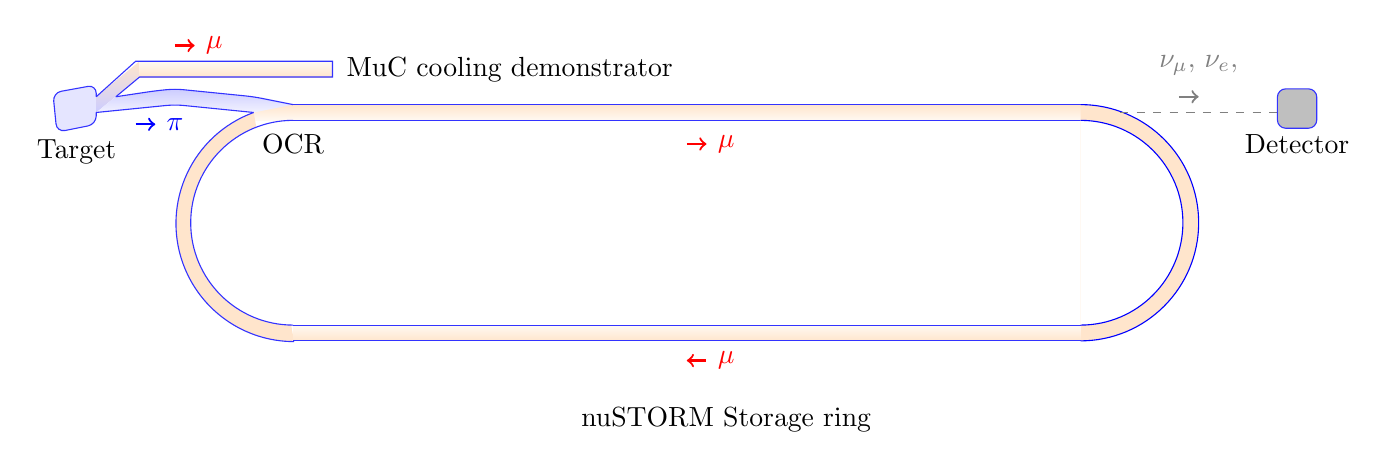
\begin{tikzpicture}[scale=0.05]
% target
\draw[blue!80, rounded corners=3pt, fill=blue!10] (10,-2) -- (10,-5) -- (0,-7) -- (-1,3) -- (10,5) -- (10, 2);
\node[] at (5,-12) {Target};


%Demo
\shade[bottom color=blue!20,top color=orange!20] (10,-2) -- (21,7) -- (21,11) -- (10,2);
\shade[bottom color=orange!20,top color=orange!5] (70,11) -- (70,7) -- (21, 7) -- (21, 11);
\draw[blue!80] (10,2) -- (20,11) -- (70,11) -- (70,7) -- (21, 7) -- (15, 2);
\node[] at (115,9) {MuC cooling demonstrator};
\draw[thick,->, color=red] (30,15) -- (35,15);
\node[text=red] at (40,15) {$\mu$};

% storage ring
\shade[top color=orange!20, bottom color=orange!5] (50, 0) -- (260,0) -- (260,-4) -- (50, -4);
\draw[blue!80, fill=orange!20] (50,-2) arc (110:270:30);
\draw[blue!80, fill=white] (60,-4) arc (90:270:26);
\draw[blue!80] (60, 0) -- (260,0);
\draw[blue!80] (60, -4) -- (260,-4);
\draw[blue, fill=orange!20] (260,-60) arc (-90:90:30);
\draw[blue, fill=white] (260,-56) arc (-90:90:26);
\shade[top color=orange!5, bottom color=orange!20] (60, -56) -- (260,-56) -- (260,-60) -- (60, -60);
\draw[blue!80] (60, -56) -- (260,-56);
\draw[blue!80] (60, -60) -- (260,-60);
\draw[thick,->, color=red] (160,-10) -- (165,-10);
\node[text=red] at (170,-10) {$\mu$};
\draw[thick,<-, color=red] (160,-65) -- (165,-65);
\node[text=red] at (170,-65) {$\mu$};
\node[] at (170,-80) {nuSTORM Storage ring};

%Pion line
\shade[bottom color=blue!5,top color=blue!20] (15, 2) -- (25,3.5) -- (30,4) -- (35,3.5) -- (50,2) -- (60,0) -- (50,-2) -- (35,-0.5) -- (30,0) -- (25,-0.5) -- (10, -2);
\draw[blue!80, rounded corners=3pt] (15, 2) -- (25,3.5) -- (30,4) -- (35,3.5) -- (50,2) -- (60,0);
\draw[blue!80, rounded corners=3pt] (10, -2) -- (25,-0.5) -- (30,0) -- (35,-0.5) -- (50,-2);
\draw[thick,->, color=blue] (20,-5) -- (25,-5);
\node[text=blue] at (30,-5) {$\pi$};
\node[] at (60,-10) {OCR};


% detector
\draw[gray, dashed] (270,-2) -- (310, -2);
\draw[blue!80, fill=gray!50, rounded corners=3pt] (310,-6) rectangle (320,4);
\draw[thick,->, color=gray] (285,2) -- (290,2);
\node[text=gray] at (290,10) {$\nu_{\mu}$, $\nu_{e}$, };
\node[] at (315,-10) {Detector};

\end{tikzpicture}

\vspace{-20pt}
\caption{Schematic showing nuSTORM including the muon cooling demonstrator for the muon collider. \label{fig_muon:nustorm}}
\end{figure*}

%\subsubsection{Synergies on machine technologies} 
The ambitious programme of R\&D necessary to deliver the muon collider has the potential to enhance the science that can be done at other muon-beam facilities. The progress in other accelerator facilities will also benefit the design and construction of the muon collider in the future.

nuSTORM \cite{Ahdida:2020whw} and ENUBET \cite{Delogu:2022yqp} offer world-leading precision in the measurement of neutrino cross sections and exquisite sensitivity to sterile neutrinos and physics beyond the Standard Model. nuSTORM in particular will require capture and storage of a high-power pion and muon beam and management of the resultant radiation near to superconducting magnets. In nuSTORM, multi-GeV pions are brought from a target and injected into a racetrack-shaped storage ring. The storage ring is tuned to capture muons arising from pions that decay in the first straight. Remnant pions are extracted to a beam dump, while the muons are circulated many times. The apparatus would deliver a `flash' of neutrinos from the initial pion decay followed by a well-characterised neutrino beam arising from the decay of the circulating muon beam. The momentum of the circulating muon beam, and hence the resultant neutrinos, would be tunable, enabling characterisation of neutrino interactions with the detector over a broad range of momenta.

The muon rate and energy for nuSTORM as compared to the muon collider and other muon beamlines is shown in Figure~\ref{fig_muon:power}. The target and capture system for nuSTORM and ENUBET may also provide a testing ground for the technologies required at the muon collider and as a possible source of beams for the essential 6D cooling-demonstration experiment, for example as in the schematic shown in Figure~\ref{fig_muon:nustorm}.

The ongoing LBNF and T2HK projects and their future upgrades will develop graphite targets to sustain the bombardment of MW-level proton beams, which may also lead to a solution for the muon production target for the muon collider. The next generation searches for charged lepton flavour violation exploit high-power proton beams impinging on a solid target placed within a high-field solenoid, such as COMET at J-PARC and Mu2e at FNAL. The technological issues of target and muon capture for these experiments are similar to those present in the muon collider design.

 The potential to deliver high quality muon beams could enhance the capabilities of muon sources such as those at PSI, J-PARC and ISIS. The use of frictional cooling to deliver ultra-cold positive and negative   muon beams is under study at PSI and may be applicable to the muon collider.

High-power proton accelerators are in use throughout the world, accelerating protons using linacs and accumulation in fixed energy rings or prior to further acceleration using rapid cycling synchrotrons. Proton drivers having power ranging from hundreds of kW to multiple MW are used as spallation neutron sources at SNS, J-PARC, ESS, PSI, ISIS and CSNS and neutrino sources at FNAL and J-PARC proton accelerator complexes as well accelerator-driven systems such as CiADS and MYRRHA. Many of the accelerator technologies required for the muon collider proton beam and for rapid acceleration are in use or under development at these facilities. For example FFAs have been proposed as a route to attain high proton beam power for secondary particle sources such as neutron spallation sources, owing to the potential for high repetition rate and lower wall plug power compared to other accelerator schemes. 

The underlying technologies required for the muon collider are also of interest in many scientific fields. The delivery of high field solenoid magnets is of great interest to fields as wide ranging as particle physics, accelerator science and imaging technology. Operation of RF cavities with high gradient is of interest to the accelerator community.

\subsection{Outlook}\label{sec:conc_out}
The muon collider presents enormous potential for fundamental physics at the energy frontier.
Previous studies  have demonstrated feasibility of many critical components  of the facility. Several proof-of-principle experiments and component tests like MICE,
CBETA, EMMA and the MUCOOL programme, have been carried out to practically demonstrate the underlying
technologies. 
Bright muon beams are also the basis of the nuSTORM facility. This experiment could share a large part of the complex with a cooling demonstrator.

The muon collider is a novel concept and is not as mature as the other high-energy lepton
collider options. However, it promises a
unique opportunity to deliver physics reach at the energy frontier on a cost, power consumption and time
scale that might improve significantly on other energy-frontier colliders. At this stage, building
upon significant prior work, no insurmountable technological issues were identified.
Therefore a development path can address the major challenges and deliver
a 3~\TeV muon collider by 2045. 

A global assessment has identified the R\&D effort that is essential to
address these challenges before the next regional strategy processes to a level that allows estimation of the performance, cost and power consumption with adequate certainty.   Execution of this R\&D is required in order to
maintain the timescale described in this document.  Ongoing developments in underlying technologies
will be exploited as they arise in order to ensure the best possible performance.  This R\&D effort will
allow future strategy processes to make fully informed recommendations.  Based on the subsequent decisions, a significant ramp-up of resources could
be made to accomplish construction by 2045 and exploit the enormous potential of the muon collider.